%% Springer Nature journal template (sn-jnl), numbered references.
%% DRAFT: every number in the Results section is a placeholder (\tbd) until the experiments are run.
\documentclass[pdflatex,sn-mathphys-num]{sn-jnl}

\usepackage{graphicx}
\usepackage{multirow}
\usepackage{amsmath,amssymb,amsfonts}
\usepackage{amsthm}
\usepackage{mathrsfs}
\usepackage[title]{appendix}
\usepackage{xcolor}
\usepackage{textcomp}
\usepackage{manyfoot}
\usepackage{booktabs}
\usepackage{algorithm}
\usepackage{algorithmicx}
\usepackage{algpseudocode}
\usepackage{listings}

\newcommand{\tbd}[1][TBD]{\textcolor{red}{#1}}   % placeholder for results not yet measured
\newcommand{\ESP}{\mathrm{ESP}}
\newcommand{\UCR}{\mathrm{UCR}}
\newcommand{\ER}{\mathrm{ER}}
\newcommand{\IoU}{\mathrm{IoU}}

\theoremstyle{thmstyleone}
\newtheorem{definition}{Definition}

\raggedbottom

\begin{document}

\title[Evidence-Grounded Reliability of CXR VLMs under Shift]{Evidence-Grounded Reliability Evaluation of Vision-Language Models for Chest X-ray Interpretation under Distribution Shift}

% Author list copied from the OGR paper; change it if the supervisors for this work are different.
\author*[1]{\fnm{} \sur{Lakshya}}\email{lakshya.2502010001@muj.manipal.edu}
\author[1]{\fnm{Amit Kumar} \sur{Bairwa}}
\author[1]{\fnm{Varun} \sur{Tiwari}}

\affil*[1]{\orgdiv{Department of Artificial Intelligence and Machine Learning, School of Computer Science and Engineering}, \orgname{Manipal University Jaipur}, \orgaddress{\street{Jaipur--Ajmer Express Highway}, \city{Jaipur}, \postcode{303007}, \state{Rajasthan}, \country{India}}}

\abstract{Vision-language models (VLMs) now write chest X-ray (CXR) reports, and some also return a box for each finding. Their reliability is still measured almost entirely by comparing the generated report with a reference report written at the same hospital. Under distribution shift this comparison is confounded, because a change of hospital changes the reporting style as well as the images, so a drop in a reference-based score cannot be separated from a change in how reports are written. We propose an evaluation that checks every positive finding a VLM claims against independent image evidence: bounding boxes drawn by expert radiologists. We define the Evidence-Support Precision (ESP), the share of claimed findings that are supported by expert evidence in the same image, together with its complement, the unsupported-claim rate, and evidence recall. We use the agreement of a claim's localisation across sampled generations as a confidence signal for abstention. We evaluate open VLMs that localise their own findings (CheXagent-2, Qwen2.5-VL and Lingshu, with MedGemma~1.5 and MAIRA-2 added once access is granted) on six public sites from three countries (USA, China and India) and under five families of image corruption at two severities. We introduce an evidence-ablation test that removes the expert-marked regions from the image, against a control that removes equal areas elsewhere in the lungs, to measure whether a claim depends on its evidence at all. We further test whether conformal claim filters calibrated at one site keep their guarantee at others, and propose a training-free self-grounding filter whose threshold is recalibrated at a new hospital from a few dozen labelled images. \tbd[Results summary to be written after the experiments.] Code, prompts and label mappings will be released.}

\keywords{Vision-language models, Chest X-ray, Radiology report generation, Grounding, Hallucination, Distribution shift, Calibration, Selective prediction, Conformal prediction}

\maketitle

%=====================================================================
\section{Introduction}\label{sec:intro}
%=====================================================================

Chest radiography is the most frequently performed imaging examination, and automatic report generation is one of the most studied applications of medical vision-language models (VLMs). In the last two years the field has moved from text-only generators such as LLaVA-Med~\cite{llavamed}, RadFM~\cite{radfm}, LLaVA-Rad~\cite{llavarad} and CheXagent~\cite{chexagent} to models that attach spatial evidence to what they say. MAIRA-2 produces a list of sentence--box pairs~\cite{maira2}, MedGemma~1.5 adds anatomical bounding-box localisation~\cite{medgemma15}, and RadVLM~\cite{radvlm} and AnatomiX~\cite{anatomix} ground phrases in the image. General-purpose models such as Qwen2.5-VL~\cite{qwen25vl} also return boxes natively.

The way these models are evaluated has not kept pace. Almost every report-quality metric compares the generated report with a reference report: CheXbert F1~\cite{chexbert}, RadGraph F1~\cite{radgraph}, RadCliQ~\cite{radcliq}, GREEN~\cite{green}, RaTEScore~\cite{ratescore} and FineRadScore~\cite{fineradscore}. RadFact, introduced with MAIRA-2, adds a spatial check, but again against reference boxes from the same distribution~\cite{maira2}. Reference-free hallucination detectors exist, but they rely on model-internal signals rather than on the image~\cite{rextrust,semcons}. FactCheXcker re-examines the image only for quantitative measurements such as tube position~\cite{factchexcker}.

This dependence on reference text becomes a problem when a model is moved to a new hospital, which is the situation that matters for deployment. The CXR literature has shown repeatedly that models degrade across sites~\cite{zech,degrave} and across patient groups~\cite{underdiag}. For VLMs the evidence is growing. Weak image artefacts reduced CXR accuracy by 10.46\% on average, and models flagged strong artefacts in only 11.5\% of cases~\cite{artefacts}. Report quality falls on out-of-distribution sets~\cite{hoppr,lrrg}, and clinician preference for Flamingo-CXR reports was 56.1\% for intensive-care films against 77.7\% for outpatient films~\cite{flamingocxr_nm}. But when MAIRA-2 was evaluated on PadChest, its lexical scores were far below its clinical scores, which the authors attributed partly to a different report structure~\cite{maira2}. The choice of reference report alone changes the scores~\cite{reportingpractice}, and Med-Gemini did not report RadGraph F1 on its Indian test set because the metric is tuned to MIMIC-style reports~\cite{medgemini}. When the site changes, a reference-based metric cannot tell whether the model got worse or the reports were written differently.

Expert boxes do not have this problem. A box drawn by a radiologist around a pneumothorax is evidence about the image, not about how a report is phrased, and it means the same thing at every hospital. Several public CXR datasets provide such boxes~\cite{chestxdet,nih14,vindr,padchestgr}, but they have been used to score phrase grounding within one distribution rather than to check the faithfulness of generated reports across distributions.

At the same time, reliability benchmarks for medical VLMs have multiplied~\cite{cares,probmed,medvh,medhallmark,medhallbench,medheval,surevqa,medqdeg,hallucxr,mvcbench,mccxr}, and calibration and abstention methods have been adapted to medical generation~\cite{semcons,conffact,confalign,score,adaptcal,conrep}. The closest prior studies each cover at most two of the three ingredients that matter here: evidence checks, controlled shift, and calibration under that shift. Predictive entropy has been shown to support selective prediction from MIMIC to PadChest, but for binary questions, without grounding~\cite{entropyshift}. HalluCXR measures hallucination on MIMIC only~\cite{hallucxr}. MVC-Bench measures calibration under domain shift for contrastive classifiers~\cite{mvcbench}. RadFact checks grounding but not shift or calibration~\cite{maira2}. Grounded dual-state calibration ties confidence to visual support through counterfactual image substitution in VQA~\cite{dualread}.

This paper combines the three. Our contributions are:
\begin{enumerate}
\item An image-evidence faithfulness metric for generated CXR reports, Evidence-Support Precision (ESP), with the unsupported-claim rate and evidence recall, computed against expert boxes and independent of reference reports (Section~\ref{sec:metrics}).
\item A multi-site, multi-severity evaluation of grounding and faithfulness for open CXR VLMs that localise findings natively or on request, including label-level probes on Indian hospital data (Sections~\ref{sec:setup}--\ref{sec:results}).
\item An evidence-ablation test: the expert-marked regions are replaced by contralateral or blurred tissue, and the change in claims and yes/no probabilities is compared with a matched control that edits equal-sized lung regions without evidence. The difference, the \emph{evidence-dependence index}, separates claims that rest on the marked findings from claims the model would make anyway (Section~\ref{sec:ablation}).
\item A comparison of evidence-based and uncertainty-based abstention under shift, a test of whether conformal claim filters calibrated at one site keep their coverage at other sites, and a training-free \emph{self-grounding filter} that combines sample agreement, the yes/no probe and box agreement, with its threshold recalibrated at the target site from $m\in\{10,25,50\}$ labelled images (Section~\ref{sec:reliability}).
\item Released code, prompts, and label mappings between model vocabularies and dataset annotations.
\end{enumerate}

We test four hypotheses. \textbf{H1}: drops in reference-based metrics across sites overstate or misorder the drops in ESP. \textbf{H2}: under image corruption the unsupported-claim rate rises faster than models report degraded image quality. \textbf{H3}: localisation agreement across samples is a better abstention signal than token entropy out of distribution. \textbf{H4}: conformal claim filters calibrated at one site under-cover at others, and a few dozen local labels restore coverage. \textbf{H5}: a substantial share of correct claims survives the removal of their evidence about as often as the removal of an unrelated region, so text-level correctness overstates grounding.

%=====================================================================
\section{Related work}\label{sec:related}
%=====================================================================

\paragraph{Chest X-ray vision-language models.} Contrastive models such as CheXzero~\cite{chexzero} and BiomedCLIP~\cite{biomedclip} align images with report text and give zero-shot classification and similarity heatmaps. Generative models produce free-text reports: LLaVA-Med~\cite{llavamed}, RadFM~\cite{radfm}, LLaVA-Rad~\cite{llavarad}, CheXagent~\cite{chexagent}, Lingshu~\cite{lingshu} and the Gemini-based Med-Gemini~\cite{medgemini}. Grounded report generation was introduced by MAIRA-2~\cite{maira2} and extended by RadVLM~\cite{radvlm}, AnatomiX~\cite{anatomix} and MedGemma~1.5~\cite{medgemma15}. Reinforcement-learning approaches to medical grounding have also appeared~\cite{medrpg_r1}.

\paragraph{Report evaluation and hallucination.} Report metrics range from label agreement (CheXbert~\cite{chexbert}) and entity--relation graphs (RadGraph~\cite{radgraph}) to composite and LLM-based scores (RadCliQ~\cite{radcliq}, GREEN~\cite{green}, RaTEScore~\cite{ratescore}, FineRadScore~\cite{fineradscore}). ReXrank ranks report generators on several data sources~\cite{rexrank}. Hallucination benchmarks for medical VLMs include MedVH~\cite{medvh}, Med-HallMark~\cite{medhallmark}, MedHallBench~\cite{medhallbench}, MedHEval~\cite{medheval} and, for CXR, HalluCXR~\cite{hallucxr}. ProbMed showed that adversarial probing questions push medical VLMs below random accuracy~\cite{probmed}, and CARES evaluates trustworthiness more broadly~\cite{cares}.

\paragraph{Distribution shift in chest radiography.} Site-dependent generalisation~\cite{zech}, shortcut learning~\cite{degrave} and underdiagnosis in under-served groups~\cite{underdiag} are well documented for classifiers. For VLMs, robustness has been studied under synthetic corruption~\cite{medmnistc,medimetac}, realistic artefacts~\cite{artefacts}, quality degradation~\cite{medqdeg,lrrg}, misleading context~\cite{mccxr}, and realistic VQA shifts~\cite{surevqa}. Report generation has been evaluated on held-out sources~\cite{hoppr,rexrank}, but the score changes have not been attributed to the type of shift or checked against image evidence.

\paragraph{Calibration, abstention and conformal prediction.} Semantic consistency across sampled reports identifies uncertain reports, and abstaining on the most uncertain 20\% improves factuality~\cite{semcons}. Conformal Factuality~\cite{conffact} and Conformal Alignment~\cite{confalign} filter generated claims with statistical guarantees, and selective conformal risk control has been extended to shift~\cite{score}. In medicine, conformal prediction has been applied to CXR impression drafting~\cite{conrep}. A small number of local labels has been shown to raise certified coverage in medical VQA considerably~\cite{adaptcal}, and predictive entropy transfers as a selective-prediction signal across two CXR sites~\cite{entropyshift}. MVC-Bench benchmarks calibration of medical contrastive models~\cite{mvcbench}. None of these uses expert image evidence as the definition of a correct claim. The closest counterfactual test, grounded dual-state calibration, swaps the whole image~\cite{dualread}; removing only the expert-marked region, with an equal-area control, asks a narrower question: whether the claim depends on the specific evidence.

%=====================================================================
\section{Datasets and shift axes}\label{sec:data}
%=====================================================================

Table~\ref{tab:datasets} lists the data. Expert boxes provide the evidence, and report-bearing sets let us compare ESP with reference-based metrics. Label-only sets serve as classification-style probes.

\begin{table}[t]
\caption{Datasets. \emph{Role}: E = expert box evidence, R = reference reports, L = image-level labels only. Access: O = open download, F = free registration, P = PhysioNet credentialed, Q = on request. The last three rows are added when access is granted.}\label{tab:datasets}
\centering
\scriptsize
\setlength{\tabcolsep}{3pt}\begin{tabular}{@{}p{3.2cm}lrp{2.6cm}cc@{}}
\toprule
Dataset & Country & Images & Annotation & Access & Role \\
\midrule
ChestX-Det test~\cite{chestxdet} & USA (NIH) & 553 & boxes, 13 classes & O & E \\
ChestX-Det train (calib.) & USA (NIH) & 300 & as above & O & E \\
Shenzhen~\cite{shenzhen,shenzhenroi} & China & 662 & TB; typed lesion outlines & O & E, L \\
Montgomery~\cite{shenzhen} & USA & 138 & TB label & O & L \\
IU-Xray~\cite{iuxray} & USA (Indiana) & 500 & reports & O & R \\
Mendeley CXR~\cite{mendeleyin} & India (3 hospitals) & 400 of 799 & COVID / abnormal / normal & O & L \\
NITRD TB A/B~\cite{nitrd} & India (New Delhi) & 306 & TB / non-TB, 2 scanners & O & L \\
\midrule
MIMIC-CXR + MS-CXR~\cite{maira2} & USA (Boston) & \tbd & reports, phrase boxes & P & R, E \\
VinDr-CXR~\cite{vindr} & Vietnam & \tbd & boxes, 22 findings & P & E \\
PadChest-GR~\cite{padchest,padchestgr} & Spain & \tbd & grounded reports & Q & R, E \\
\botrule
\end{tabular}
\end{table}

\paragraph{Site.} Each source is treated as a site. The two evidence sites differ in country, scanner and annotation protocol. In ChestX-Det the boxes of 13 classes are mapped to the shared space $\mathcal{F}$; calcification, emphysema and fibrosis have no counterpart and support only the generic \emph{opacity} claim. In Shenzhen, two radiologists outlined every lung lesion of the TB-positive films and named its type~\cite{shenzhenroi}; infiltrates map to consolidation, nodules and cavities to nodule/mass, and effusion and apical, interlobar or other pleural thickening to their counterparts. Normal Shenzhen films have no lesions, so every finding is absent there; on TB films the heart and bones were not reviewed, so cardiomegaly and fracture claims are excluded as unverifiable. Indian data have image-level labels only and are evaluated as a normal/abnormal or TB probe (accuracy, calibration and selective risk), not with ESP. MIMIC-CXR is the in-distribution anchor because most models were trained on it; MS-CXR is reported separately for models that saw it in training (MAIRA-2, RadVLM).

\paragraph{Image quality.} Following MedMNIST-C~\cite{medmnistc}, we apply five corruption families at a mild and a severe level to 100 images from each evidence site: additive Gaussian noise ($\sigma=0.04, 0.16$ on a $[0,1]$ scale), Gaussian blur ($\sigma=1, 4$ pixels per 512 pixels of image size), JPEG compression (quality 30, 5), contrast reduction (factor 0.6, 0.25 around mid-grey) and rotation ($5^\circ, 20^\circ$). Expert boxes are rotated with the image.

\paragraph{Acquisition and demographics.} View position (AP vs.\ PA, portable vs.\ fixed) and sex and age groups are analysed once CheXpert Plus and MIMIC-CXR, which carry this metadata, are added. Within the open sites, NITRD Datasets A and B were acquired on two different scanners.

%=====================================================================
\section{Method}\label{sec:method}
%=====================================================================

\subsection{Models}\label{sec:models}

We evaluate open models that fit on one 16\,GB GPU (Table~\ref{tab:models}). All of them return boxes as text, so a claim can be localised by asking the model to locate the claimed finding. CheXagent-2 was trained to emit boxes on a $0$--$100$ grid and sometimes grounds its report sentences directly; Qwen2.5-VL emits JSON boxes in pixel coordinates; Lingshu shares the Qwen2.5-VL architecture but was not evaluated on medical grounding by its authors, so its boxes test whether the format alone transfers. MedGemma~1.5 and MAIRA-2 are gated and are added when access is granted. Post-hoc saliency for text-only models is left for future work. CheXagent-2's instruction data include NLM-TB (Shenzhen and Montgomery), OpenI (IU-Xray) and ChestX-ray14, from which the ChestX-Det images are drawn~\cite{chexagent}; for this model only the two Indian sites are unseen hospitals, and results on the other sites are read with that in mind. The training data of the Qwen-family models are not published.

\begin{table}[t]
\caption{Models. Precision is the numeric format used for inference.}\label{tab:models}
\centering
\footnotesize
\begin{tabular}{@{}lllll@{}}
\toprule
Model & Parameters & Box output & Precision & Licence \\
\midrule
CheXagent-2~\cite{chexagent} & 3B & native, $0$--$100$ grid & bf16 & MIT \\
Qwen2.5-VL~\cite{qwen25vl} & 7B & native, JSON pixels & 4-bit NF4 & Apache-2.0 \\
Lingshu~\cite{lingshu} & 7B & prompted, JSON pixels & 4-bit NF4 & MIT \\
MedGemma 1.5~\cite{medgemma15} & 4B & native & bf16 & HAI-DEF terms (pending) \\
MAIRA-2~\cite{maira2} & 7B & native, grounded report & 8-bit & research only (pending) \\
\botrule
\end{tabular}
\end{table}

\subsection{Claim extraction}\label{sec:claims}

For image $x$, model $m$ generates a findings section $r$. A CheXbert labeller~\cite{chexbert} run locally extracts the set of positive findings. Each finding $f$ is mapped to a shared label space $\mathcal{F}$ (atelectasis, cardiomegaly, consolidation, oedema, effusion, pneumonia, pneumothorax, opacity, nodule/mass), using hand-built mappings to each dataset's label set (Appendix~\ref{app:mapping}). If the model localises a finding, we attach its box $\hat b$. Grounding tags in CheXagent-2 output are removed before labelling. This gives the claim set
\begin{equation}
C_m(x) = \{(f_j, \hat b_j)\}_{j=1}^{|C_m(x)|}, \qquad f_j \in \mathcal{F},\; \hat b_j \in \mathcal{B}\cup\{\varnothing\}.
\end{equation}
We check \tbd[200] extracted claims by hand and report the extraction error rate. Uncertain mentions (``possible effusion'') are recorded but not counted as claims.

\subsection{Evidence-support metrics}\label{sec:metrics}

Let $E(x)=\{(f, B_f)\}$ be the expert evidence for image $x$, where $B_f$ is the set of expert boxes for finding $f$. We assume that, within $\mathcal{F}$, the annotation is exhaustive: a finding without a box is absent.

\begin{definition}[Supported claim]
A claim $(f_j,\hat b_j)$ is supported by $E(x)$ if $f_j$ has at least one expert box and, when $\hat b_j\neq\varnothing$, $\max_{B\in B_{f_j}} \IoU(\hat b_j, B)\ge\tau$. The pointing variant replaces the IoU test by requiring the centre of a predicted box to lie inside an expert box.
\end{definition}

Over a set of images $X$,
\begin{align}
\ESP_m &= \frac{\sum_{x\in X} \big|\{c\in C_m(x): c \text{ supported}\}\big|}{\sum_{x\in X} |C_m(x)|}, \qquad \UCR_m = 1-\ESP_m, \\
\ER_m &= \frac{\sum_{x\in X} \big|\{f: B_f\neq\varnothing,\; f \text{ claimed and supported}\}\big|}{\sum_{x\in X} \big|\{f: B_f\neq\varnothing\}\big|}.
\end{align}
We report $\tau\in\{0.3, 0.5\}$, and a text-only variant ($\tau=0$) that ignores location. We also report standard grounding scores (mIoU, accuracy at IoU $0.3$ and $0.5$, pointing game) and, where reference reports exist, CheXbert F1, RadGraph F1 and GREEN. On corrupted images we record the \emph{artefact-awareness rate}: the share of reports that mention degraded image quality.

\subsection{Evidence ablation}\label{sec:ablation}

For an image with expert evidence, the \emph{evidence-removed} version replaces every expert box by the mirrored region of the opposite hemithorax, or by a heavily blurred copy of the image (Gaussian, $\sigma = 0.08$ of the image size) when the mirrored region holds a lesion too. The \emph{control} version applies the same fill to boxes of the same sizes placed at random inside the lung zones (left and right of the mediastinum, $10$--$82\%$ of the image height) so that they touch no expert box. Only images for which every control box can be placed are used, so both versions edit the same number of boxes of the same sizes. For every finding $f$ with evidence that the model claims on the clean image, we record whether the claim survives each edit, and for every evidenced finding the drop in the yes/no probability $\Delta p_f$. The evidence-dependence index is
\begin{equation}
\mathrm{EDI} = \Pr[\text{claim lost} \mid \text{evidence removed}] - \Pr[\text{claim lost} \mid \text{control}],
\end{equation}
and analogously for $\Delta p_f$. An EDI near zero means the model's claims and confidence are insensitive to the specific evidence, even when the claims are correct.

\subsection{Confidence signals and abstention}\label{sec:reliability}

For every claim we compute four confidence scores: (i) the probability of the claim sentence, the exponential of its mean token log-probability in the greedy report; (ii) semantic consistency, the share of $K$ sampled reports that contain the same finding~\cite{semcons}; (iii) a yes/no probe, the probability the model gives to ``yes'' against ``no'' when asked whether the image shows the finding; and (iv) \emph{evidence consistency},
\begin{equation}
s_{\mathrm{ev}}(f) = \frac{1}{K}\sum_{k=1}^{K}\mathbb{1}[f\in C^{(k)}]\;\cdot\;\overline{\IoU}\big(\hat b^{(k)}_f, \hat b^{(k')}_f\big),
\end{equation}
computed over one greedy and $K'$ sampled localisation requests for $f$: it multiplies the share of requests that return a box by the mean pairwise IoU of the returned boxes. The \emph{self-grounding score} is the mean of (ii), (iii) and (iv), the three signals that condition on the image rather than on the generated text alone.

With a claim counted correct when it is supported at the text level, we report expected calibration error (ECE), Brier score, area under the risk--coverage curve (AURC), and selective risk at 80\% and 90\% coverage, for each site and severity.

\paragraph{Conformal transfer.} Following Conformal Factuality~\cite{conffact}, for each calibration report we take the smallest threshold on the confidence score above which every retained claim is supported. The $(1-\alpha)$ quantile $\hat q$ of these thresholds, computed on held-out ChestX-Det training images, guarantees under exchangeability that a filtered report contains no unsupported claim with probability at least $1-\alpha$. We compute $\hat q$ there and measure the realised coverage and the retained-claim fraction at every other site and severity, for $\alpha\in\{0.05, 0.1, 0.2\}$. For the \emph{site-adaptive} variant, $\hat q$ is recomputed from $m$ randomly drawn labelled images of the target site and evaluated on the remaining images of that site (200 random draws per $m$).

\begin{algorithm}[t]
\caption{Evaluation protocol for one model $m$ (corruption runs; ablation runs replace $c$ by the evidence or control edit)}\label{alg:protocol}
\begin{algorithmic}[1]
\For{each site $s$ and corruption (family, severity) $c$, including none}
  \For{each image $x$ in the sample of site $s$}
    \State $\tilde x \gets c(x)$; transform expert boxes if $c$ is geometric
    \State generate one greedy report and $K$ sampled reports from $m(\tilde x)$
    \State extract claims $C_m(\tilde x)$; ask for boxes of each claimed or expert-evidenced finding
    \State compute the four confidence scores for each claim
  \EndFor
  \State compute ESP, UCR, ER, grounding, reference-based scores and calibration on $(s,c)$
\EndFor
\State calibrate a conformal threshold on the calibration site; measure coverage on all $(s,c)$
\end{algorithmic}
\end{algorithm}

%=====================================================================
\section{Experimental setup}\label{sec:setup}
%=====================================================================

All sites use every image except Mendeley (400 of 799, drawn with a fixed seed) and IU-Xray (500 studies with a findings section; IU-Xray has no view metadata, so the frontal image of each study is the one BiomedCLIP~\cite{biomedclip} rates most likely to be frontal in a zero-shot test, and studies without a likely frontal image are skipped). Images are resized so that the longer side is at most 1024 pixels. For each image a model writes one greedy report and, on evidence sites, $K=5$ sampled reports (temperature 0.7, top-$p$ 0.95). Each finding that is claimed or has expert evidence is localised once greedily and $K'=3$ times by sampling. The model also answers a yes/no question for each finding in $\mathcal{F}$ and three further questions (is the image normal, does it show tuberculosis, is the image quality adequate). On label-only sites no reports are sampled and no boxes are requested. The corruption grid uses 100 images per evidence site with $K=3$ and $K'=2$; the evidence-ablation runs use every matched image with $K=3$ and no localisation requests. The yes/no probes of the Qwen-family models are computed in left-padded batches; on 30 images with 12 questions each, batching changes $P(\text{yes})$ by 0.005 on average and by at most 0.031 for either model, compared with asking each question alone. Prompts are listed in Appendix~\ref{app:prompts}. All runs use one NVIDIA RTX 5070 Ti (16\,GB) with PyTorch~2.9 and Transformers~4.57 (4.40 for CheXagent-2, as its code requires). Differences between models and between sites are tested with paired bootstrap confidence intervals over images (1{,}000 resamples). Closed commercial models are not evaluated on credentialed data, in keeping with the PhysioNet data use agreement.

%=====================================================================
\section{Results}\label{sec:results}
%=====================================================================

\noindent\tbd[Partial results: CheXagent-2 is complete on the evidence sites, Montgomery and Mendeley; Qwen2.5-VL on both evidence sites and Montgomery; Lingshu on ChestX-Det and 396 of 662 Shenzhen images. The Qwen-family ablations, NITRD, IU-Xray, the calibration split and the corruption grid are running.]

\subsection{Evidence support across sites (H1)}

\begin{table}[t]
\caption{Evidence support on clean images: Evidence-Support Precision at the text level (ESP, with 95\% bootstrap interval) and with the model's own box overlapping an expert box (ESP@0.3), evidence recall (ER), and oracle grounding mIoU. Values in \%. \tbd[Filled automatically from the experiment logs; partial until all runs finish.]}\label{tab:esp}
\centering
\scriptsize
\setlength{\tabcolsep}{3pt}
\begin{tabular}{@{}lcccccccc@{}}
\toprule
& \multicolumn{4}{c}{ChestX-Det (USA)} & \multicolumn{4}{c}{Shenzhen (China)} \\
\cmidrule(lr){2-5}\cmidrule(lr){6-9}
Model & ESP & ESP@0.3 & ER & mIoU & ESP & ESP@0.3 & ER & mIoU \\
\midrule
\csname @@input\endcsname generated/tab_esp.tex 
\botrule
\end{tabular}
\end{table}

Moving from ChestX-Det to Shenzhen, CheXagent-2's evidence-support precision falls from 64.9\% [62--68] to 55.5\% [50--60] and its evidence recall from 37.6\% to 16.3\%, while the box criterion changes much less (ESP@0.3 37.8\% vs.\ 34.8\%, mIoU 0.26 vs.\ 0.24): at the TB site the model claims fewer of the marked lesions and more findings without evidence, but the claims it does support are localised about as well. On ChestX-Det the two general-domain models reach a similar text-level precision (Qwen2.5-VL 59.8\% [54--66], Lingshu 63.6\% [59--68]) with lower evidence recall (8.9\% and 17.8\%). The shift to the TB site hurts them far more than CheXagent-2: Qwen2.5-VL falls to 24.3\% [17--32] with an evidence recall of 3.3\%, and Lingshu to 50.0\% [37--63] \tbd[(partial)]. The site ranking under ESP therefore changes with the model, and the general-domain model that is best on ChestX-Det is the worst at the TB site. Text-level and box-level support differ by 17--41 points for every model, so a claim that names the right finding is often not placed on it.

\tbd[Compare the site ranking under ESP with the ranking under reference-based metrics (CheXbert F1 on IU-Xray; RadGraph F1 and GREEN once MIMIC-CXR and PadChest-GR are added).]

\subsection{Image corruption and artefact awareness (H2)}

\begin{figure}[t]
\centering
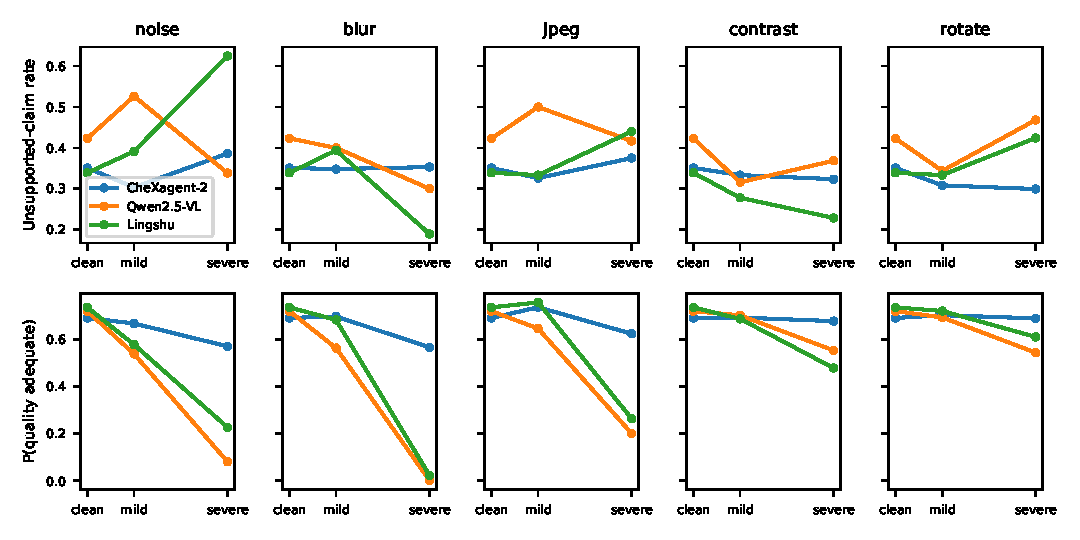
\includegraphics[width=\textwidth]{generated/fig_corruption.pdf}
\caption{ChestX-Det under five corruptions at a mild and a severe level: unsupported-claim rate (top) and share of reports that mention image quality (bottom). \tbd[Partial until all runs finish.]}\label{fig:corruption}
\end{figure}

\tbd[Describe Fig.~\ref{fig:corruption}.]

\subsection{Abstention under shift (H3)}

\begin{table}[t]
\caption{Separating supported from unsupported claims: AUROC / AURC of each confidence signal on clean images (higher AUROC and lower AURC are better). \tbd[Partial until all runs finish.]}\label{tab:calib}
\centering
\scriptsize
\setlength{\tabcolsep}{3pt}
\begin{tabular}{@{}llccccc@{}}
\toprule
Model & Site & Sent.\ prob. & Agreement & Yes/no & Box agr. & Self-ground. \\
\midrule
\csname @@input\endcsname generated/tab_calib.tex 
\botrule
\end{tabular}
\end{table}

The sentence probability, the signal most often used to flag hallucinated sentences, separates supported from unsupported claims worst in all six model--site settings (AUROC 0.10--0.47). It is below chance throughout and far below for Qwen2.5-VL (0.25 on ChestX-Det, 0.10 on Shenzhen): the sentences that model writes most confidently are more often unsupported. The yes/no probe is the best single signal in five of six settings (0.66--0.88) and stays strong under the site shift. Box agreement is useful only for the model trained to ground (CheXagent-2, 0.62--0.70; 0.35--0.57 for the others). The self-grounding score, which averages the probe with sample and box agreement, is the best signal for CheXagent-2 on ChestX-Det (0.71, ECE 0.05) but inherits the weakness of box agreement for the general-domain models (0.49 for Lingshu on Shenzhen against 0.77 for the probe). The probe alone is therefore the safer default; box agreement should enter the score only for models with a grounding objective. \tbd[Same comparison on corrupted images.]

\subsection{Conformal transfer (H4) and the site-adaptive filter}

\begin{figure}[t]
\centering
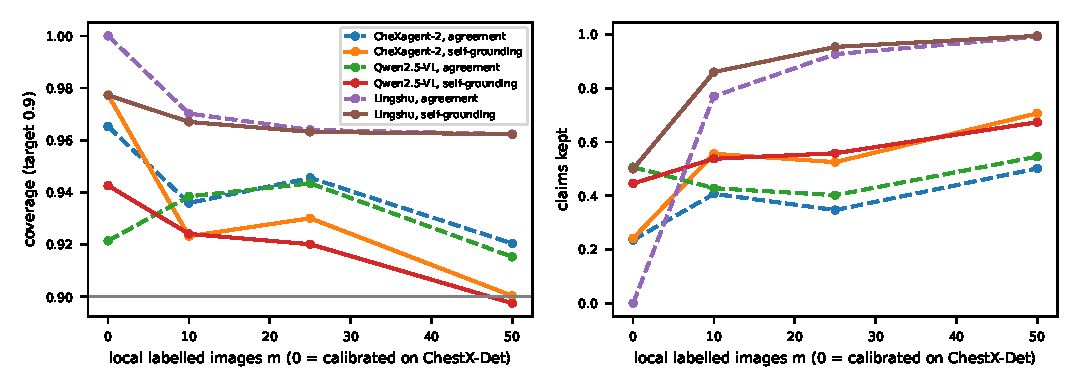
\includegraphics[width=\textwidth]{generated/fig_local.pdf}
\caption{Claim filter on Shenzhen at target coverage $0.9$ ($\alpha=0.1$): realised coverage (left) and share of claims kept (right) when the threshold is calibrated on ChestX-Det ($m=0$) or on $m$ labelled Shenzhen images. \tbd[Partial until all runs finish.]}\label{fig:local}
\end{figure}

\tbd[Describe Fig.~\ref{fig:local}.]

\subsection{Evidence dependence (H5)}

\begin{table}[t]
\caption{Evidence ablation. Claims made on the clean image that are lost when the expert-marked regions are removed (Evidence) or when equal areas elsewhere in the lungs are removed (Control); their difference (EDI); and the evidence-dependence index of the yes/no probability with its 95\% bootstrap interval. \tbd[Filled when the ablation runs finish.]}\label{tab:ablation}
\centering
\scriptsize
\setlength{\tabcolsep}{3pt}
\begin{tabular}{@{}llrcccl@{}}
\toprule
Model & Site & Claims & Lost (evidence) & Lost (control) & EDI & EDI of $p$ \\
\midrule
\csname @@input\endcsname generated/tab_ablation.tex 
\botrule
\end{tabular}
\end{table}

Removing the expert-marked regions removes most of the claims that rest on them: CheXagent-2 drops 75.6\% of its evidenced claims on ChestX-Det and 73.7\% on Shenzhen, against 22.5\% and 15.8\% when regions of the same sizes are edited elsewhere in the lungs. The evidence-dependence index is 0.53 and 0.58 on claims and 0.187 [0.170, 0.207] and 0.212 [0.194, 0.230] on the yes/no probability, so the model's claims depend on the marked evidence. Two findings qualify this. About a quarter of the evidenced claims (24.4\% and 26.3\%) survive the removal of all their evidence, so they are made without it, and between 16\% and 23\% of claims disappear after an edit that touches no evidence, so a sizeable share of claims is unstable under any local change to the image. Text-level correctness counts both groups as correct.

\subsection{Label-level probes, including Indian hospital data}

\begin{table}[t]
\caption{Label-level probes from the yes/no questions: AUROC and accuracy of P(TB) or P(abnormal) $=1-$P(normal), calibration error of the answer confidence, and accuracy of the claims in the generated report (abnormal if any finding is claimed). \tbd[Partial until all runs finish.]}\label{tab:probes}
\centering
\scriptsize
\setlength{\tabcolsep}{3pt}
\begin{tabular}{@{}lllcccc@{}}
\toprule
Model & Site & Label & AUROC & Acc. & ECE & Report acc. \\
\midrule
\csname @@input\endcsname generated/tab_probes.tex 
\botrule
\end{tabular}
\end{table}

CheXagent-2 detects TB almost perfectly on Montgomery and Shenzhen (AUROC 1.00 and 0.99), but both sites are in its instruction data (Section~\ref{sec:models}), so these figures measure recall of training data rather than transfer. On the unseen Indian Mendeley site its probability of an abnormal film is barely informative (AUROC 0.58, accuracy 51.7\%) and poorly calibrated (ECE 0.36). For Qwen2.5-VL, whose training data are not published, TB detection is moderate on both public TB sites (AUROC 0.71 on Montgomery, 0.66 on Shenzhen) and poorly calibrated (ECE 0.41 and 0.50); Lingshu reaches 0.82 on Shenzhen \tbd[(partial)]. \tbd[NITRD (unseen, TB) separates the effect of the unseen hospital from the change of task; Qwen-family results.]

%=====================================================================
\section{Discussion}\label{sec:discussion}
%=====================================================================

\tbd[Draft from the CheXagent-2 and Qwen2.5-VL results; to be revised when all models and sites are in.]

\paragraph{Correct is not the same as grounded.} Three measurements separate a claim that names the right finding from a claim that rests on the evidence for it. About 25 points separate text-level from box-level support, so the model often names a finding it does not place on the marked region. A quarter of evidenced claims survive the removal of all their evidence, so they are made without it. And between 16\% and 23\% of claims vanish after an edit that touches no evidence, so many claims are fragile rather than wrong. Reference-based metrics, and text-level ESP itself, count all three groups as correct. The evidence ablation with a matched control is cheap (two extra reports per image, no localisation) and could be added to any grounded benchmark.

\paragraph{Which confidence to trust.} The token probability of the generated sentence, the most common hallucination signal, is below chance at separating supported from unsupported claims for every model, and strongly inverted for Qwen2.5-VL. Asking the model a direct yes/no question about the claimed finding is the most reliable signal in almost every setting and costs one forward pass per finding. Box agreement helps only for a model trained to ground; adding it to the score for other models makes the score worse. A deployment that cannot tune the signal per model should use the yes/no probe, never the sentence probability.

\paragraph{Seen and unseen hospitals.} The public TB sites are in CheXagent-2's instruction data, and its near-perfect TB detection there disappears on the unseen Indian site. Public CXR collections are reused so widely in instruction tuning that ``external validation'' on them can measure memorisation; a reliability study has to check each model's training sources and keep at least one site that no model has seen. Here, only the Indian data meet that requirement. \tbd[NITRD, Lingshu and the conformal results will complete this paragraph.]

\paragraph{Limitations.} ESP assumes the expert annotation is exhaustive within the shared label space; findings missed by annotators count against the model. The open grounding data come mostly from one source (NIH); the PhysioNet and PadChest-GR sites are needed for a multi-country evidence comparison. Indian data have labels only, so faithfulness and grounding cannot yet be measured on Indian patients. Claim extraction by an automatic labeller introduces errors, which we quantify by manual review. The 7B models run in 4-bit precision, which may change their behaviour slightly. Most models were trained on MIMIC-CXR, and MAIRA-2 and RadVLM also on MS-CXR, so their in-distribution results are reported separately.

%=====================================================================
\section{Conclusion}\label{sec:conclusion}
%=====================================================================

\tbd[To be written after the results.]

\backmatter

\bmhead{Acknowledgements}
\tbd[To be added.]

\section*{Declarations}

\begin{itemize}
\item \textbf{Funding:} \tbd[None / to be stated.]
\item \textbf{Conflict of interest:} The authors declare no competing interests.
\item \textbf{Ethics approval and consent to participate:} This study uses only publicly available, de-identified datasets under their data use agreements. No new data were collected from patients.
\item \textbf{Consent for publication:} Not applicable.
\item \textbf{Data availability:} All datasets are available from their original providers under the access terms given in Table~\ref{tab:datasets}.
\item \textbf{Code availability:} \tbd[Repository URL.]
\item \textbf{Author contribution:} \tbd[To be stated.]
\end{itemize}

\begin{appendices}

\section{Label mappings}\label{app:mapping}
\tbd[Mapping of each dataset's finding labels and each model's vocabulary to the shared label space $\mathcal{F}$.]

\section{Prompts}\label{app:prompts}
\textbf{Report.} Qwen2.5-VL and Lingshu: ``You are an expert radiologist. Write the findings section of a radiology report for this chest X-ray. Describe only what is visible in the image.'' CheXagent-2: ``Given the indication: "Routine chest radiograph.", write a structured findings section for the CXR.''

\textbf{Localisation.} Qwen2.5-VL and Lingshu: ``Locate every region showing \{finding\} in this chest X-ray. Output the bounding box coordinates in JSON format.'' CheXagent-2: ``Locate areas in the chest X-ray where \{finding\} are present, using bounding box coordinates.''

\textbf{Yes/no probes.} ``Does this chest X-ray show \{finding\}?'', ``Is this chest X-ray normal?'', ``Does this chest X-ray show signs of tuberculosis?'' and ``Is the image quality of this chest X-ray adequate for diagnostic interpretation?'', each followed by ``Answer with yes or no.''

\end{appendices}

\bibliography{references}

\end{document}
